\documentclass[12pt]{report}
\usepackage{titletoc}
\titlecontents{chapter}% <section-type>
  [0pt]% <left>
  {}% <above-code>
  {\bfseries\chaptername\ \thecontentslabel\quad}% <numbered-entry-format>
  {}% <numberless-entry-format>
  {\bfseries\hfill\contentspage}% <filler-page-format>
\usepackage{a4,amssymb,amsmath,amsfonts,mathrsfs,dsfont}
\usepackage{graphicx}  

\usepackage{latexsym,amssymb,rotate,amsmath,amsthm}
\def\newblock{\hskip .11em plus .33em minus .07em}
\renewcommand{\baselinestretch}{1}
\textheight=8.5in \textwidth=6.1in \oddsidemargin=0.15in
\evensidemargin=0.15in
\usepackage{epstopdf}
\usepackage{amsmath}
\usepackage[square,sort,comma,super,authoryear]{natbib}
\usepackage{float}

\usepackage{tabularx}
\newcommand\latex{\LaTeX{~}}
\newcommand{\bibtex}{BiBTeX{~}}


\usepackage{amssymb,mathrsfs}
\usepackage{natbib}
\usepackage{setspace}
\usepackage{url}
%\usepackage[T1]{fontenc}
%\usepackage{ulem}
\usepackage{listings}
\usepackage{xcolor}

\lstset{
	keywordstyle=\color{RoyalBlue},
	basicstyle=\scriptsize\ttfamily,
	commentstyle=\ttfamily\itshape\color{gray},
	stringstyle=\ttfamily,
	showstringspaces=false,
	breaklines=true,
	frameround=ffff,
	frame=single,
	rulecolor=\color{black},
	xleftmargin=\dimexpr\fboxsep-\fboxrule,
	xrightmargin=\dimexpr\fboxsep-\fboxrule,
    gobble = 8
}
\renewcommand\bibname{References}

\DeclareMathAlphabet{\mathpzc}{OT1}{pzc}{m}{it}
\usepackage[lmargin=3cm,rmargin=3cm,tmargin=3cm,bmargin=3.5cm]{geometry}
\usepackage{nomencl}
\usepackage{textcomp}

\author{Anusuya}
\date{July 2016}
\DeclareMathAlphabet{\mathpzc}{OT1}{pzc}{m}{it}

\begin{document}
%-------------------------------------Title Page-------------------------------



%-------------------------------------Title Page-------------------------------

%\begin{titlepage}

\begin{center}
	\Large
	\textbf{Android Dashboard for Past and Present Processes}
	
	\vspace*{32pt}
	\normalsize
	DISSERTATION
	
	\vspace*{32pt}
	\textbf{\textit{Submitted by}}
	
	\vspace*{32pt}
	\begin{flushleft}
		\hspace*{100pt}
		\large                             
		R.ANUSUYA
		\hspace*{2pt}
		\large
		CB.EN.P2CYS14002
	\end{flushleft}
	
	\vspace*{32pt}
	\normalsize
	\textit{\textbf{in partial fulfillment for the award of the degree}}
	
	\textbf{\textit{of}}
	
	\vspace*{32pt}
	MASTER OF TECHNOLOGY
	
	IN
	
	CYBER SECURITY
	
	\vspace*{32pt}
	
\includegraphics[keepaspectratio=true]{avvp_logo1}
	
	\vspace*{20pt}
	\normalsize
	TIFAC-CORE IN CYBER SECURITY
	
	\vspace*{5pt}
	AMRITA SCHOOL OF ENGINEERING
	
	\vspace*{5pt}
	\large
	\textbf{AMRITA VISHWA VIDYAPEETHAM}
	
	\vspace*{5pt}
	\normalsize
	COIMBATORE - 641 112
	
	\vspace*{10pt}
	AUGUST 2016
\end{center}

%\end{titlepage}


\clearpage

%---------------------------------End of Title Page--------------------------



%---------------------------------------------------------------------------------------
%                 Guidance
%--------------------------------------------------------------------------------------
%\begin{titlepage}

\begin{center}
	\Large
	\textbf{Android Dashboard for Past and Present Processes}
	
	\vspace*{22pt}
	\normalsize
	DISSERTATION
	
	\vspace*{12pt}
	\textbf{\textit{Submitted by}}
	
	\vspace*{12pt}
	\begin{flushleft}
		\hspace*{100pt}
		\large
		R.ANUSUYA
		\hspace*{2pt}
		\large
		CB.EN.P2CYS14002
	\end{flushleft}
	
	\vspace*{12pt}
	\normalsize
	\textit{\textbf{in partial fulfillment for the award of the degree}}
	
	\textbf{\textit{of}}
	
	
	\vspace*{22pt}
	MASTER OF TECHNOLOGY
	
	IN
	
	CYBER SECURITY
	
	\vspace*{22pt}
	Under the guidance of
	
	\vspace*{12pt}
	\textbf{Prof. Prabhaker Mateti}\\Associate Professor\\ Computer Science and Engineering\\Wright State University\\USA
	
	\vspace*{22pt}
	
\includegraphics[keepaspectratio=true]{avvp_logo1}
	
	\vspace{25pt}
	\normalsize
	TIFAC-CORE IN CYBER SECURITY
	
	\vspace*{5pt}
	AMRITA SCHOOL OF ENGINEERING
	
	\vspace*{5pt}
	\large
	\textbf{AMRITA VISHWA VIDYAPEETHAM}
	
	\vspace*{5pt}
	\normalsize
	COIMBATORE - 641 112
	
	\vspace*{5pt}
	AUGUST 2016
\end{center}

% \end{titlepage}

\clearpage
%----------------------------------------------------------------------------------------
%                 Bonafide certificate
%----------------------------------------------------------------------------------------
% \begin{titlepage}

\begin{center}
	\Large
	\textbf{AMRITA VISHWA VIDYAPEETHAM}
	
	\normalsize
	\textbf{AMRITA SCHOOL OF ENGINEERING,COIMBATORE -641 112}
	
	\vspace*{22pt}
	
\includegraphics[keepaspectratio=true]{avvp_logo1}
	
	\vspace*{22pt}
	\normalsize
	\textbf{BONAFIDE CERTIFICATE}
	
\end{center}

\begin{sloppypar}
	\noindent
	This is to certify that this dissertation entitled \textbf{``Android Dashboard for Past and Present Processes''} submitted by \textbf{R.ANUSUYA (Reg.No : CB.EN.P2.CYS14002)} in partial fulfillment of the requirements for the award of the \textbf{Degree of Master of Technology} in \textbf{CYBER SECURITY} is a bonafide record of the work carried out under my guidance and supervision at Amrita School of Engineering.
\end{sloppypar}


\vspace*{52pt}
\begin{flushleft}
	\noindent
	\textbf{Dr. Prabhaker Mateti \hspace*{165pt}Dr. M. Sethumadhavan}
	
	\vspace*{5pt}
	\noindent
	\hspace*{35pt}(Supervisor)
	\hspace*{212pt}
	(Professor and Head)
\end{flushleft}



\vspace*{20pt}
\begin{flushleft}
	\noindent
	This dissertation was evaluated by us on\ldots\ldots\ldots\ldots\ldots
\end{flushleft}

\vspace*{52pt}
\begin{flushleft}
	\noindent
	INTERNAL EXAMINER \hspace*{150pt} EXTERNAL EXAMINERS
\end{flushleft}

\clearpage

%\end{titlepage}

%----------------------------------------------------------------------------------------
%	DECLARATION PAGE
%	Your institution may give you a different text to place here
%----------------------------------------------------------------------------------------

%\begin{titlepage}

\begin{center}
	\large
	\textbf{AMRITA VISHWA VIDYAPEETHAM}
	
	\normalsize
	\textbf{AMRITA SCHOOL OF ENGINEERING,COIMBATORE}
	
	\textbf{TIFAC-CORE IN CYBER SECURITY}
	
	\vspace*{42pt}
	\normalsize
	DECLARATION
	
\end{center}

\vspace*{32pt}


\begin{sloppypar}
	\noindent
	\textbf{I, R.ANUSUYA (Reg.No: CB.EN.P2.CYS14002)} hereby declare that this final project report entitled \textbf{``Android Dashboard for Past and Present Processes''} is a record of the original work done by me under the guidance of \textbf{Prof. Prabhaker Mateti}, Associate professor, Wright State University, and this work has not formed the basis for the award of any degree / diploma / associateship / fellowship or a similar award, to any candidate in any University, to the best of my knowledge.
\end{sloppypar}

\vspace*{42pt}
\begin{flushleft}
	\noindent
	Place : Coimbatore
	
	\vspace*{10pt}
	\noindent
	Date :
	\hspace*{250pt}
	Signature of the Student
\end{flushleft}

\begin{center}
	
	\vspace*{70pt}
	COUNTERSIGNED
	
	\vspace*{50pt}
	\textbf{Dr. M. Sethumadhavan}
	
	Professor and Head, TIFAC-CORE in Cyber Security
	
\end{center}

%\end{titlepage}

\clearpage % Start a new page
%----------------------------------------------------------------------------------------
%	ACKNOWLEDGEMENTS
%---------------------------------------------------------------------------------------

\clearpage

\section*{{\centerline{\huge Abstract}}\hfill} \addcontentsline{toc}{chapter}{Abstract}
\vspace*{22pt}
\baselineskip 0.7 cm

Mobile phones are now indispensable devices. We use our smart phones
for all our day to day works. Among all the mobile operating systems, Android is
the most widely used. Though we use our Android phone
for many activities, we are unaware of the activities happening inside it. A savvy user would like to know which processes use  the
most memory and with what our apps are communicating. As of now, we do not have
any service that monitors the Android OS from within and tells what the running processes are doing and what the old processes were doing.

This thesis contributes to monitoring the Android OS
constantly. It presents a dashboard for getting the details of present and past processes. It analyses the process behavior with tools like strace and ltrace. These details are logged and are uploaded to the cloud. The logged data are analysed to provide the provenance of a process. We use Android\textquotesingle s API like RunningAppProcessInfo, Activity Manager, etc., to retrieve the details of present running processes. Android dashboard for past and present application, provides the end user with the details of all the happenings inside Android device by analysing the processes. 
The source code and related documents of this thesis are available in the link https://github.com/anurp/DashboardOfProcess

\textbf{Keywords:} Android, OS Monitor, Android Processes, Strace, ltrace. 

\baselineskip 1cm
\newtheorem{thm}{Theorem}[section]
\newtheorem{cor}[thm]{Corollary}%[section]
\newtheorem{pro}{Proposition}[section]
\newtheorem{lemma}{Lemma}%[section]
\newtheorem{rem}[thm]{Remark}%[section]
\newtheorem{note}[thm]{Note}%[section]
\newtheorem{defn}{Definition}[section]
\newtheorem{con}[thm]{Conjecture}


\pagenumbering{roman}
\newpage
\baselineskip 1 cm
%\pagenumbering{roman}
\tableofcontents

%\pagenumbering{roman}
\newpage
\baselineskip .5 cm
%\pagenumbering{roman}
\listoffigures  \addcontentsline{toc}{chapter}{List of Figures}

\newpage
\baselineskip .5 cm
%\pagenumbering{roman}
\listoftables  \addcontentsline{toc}{chapter}{List of Tables}


\newpage
\baselineskip 1cm
\pagenumbering{arabic}
\setcounter{page}{1}
\clearpage 
\chapter{Introduction}
As smartphones and tablets become more popular, the operating systems for those
devices become more important. Android is such an operating system for low
powered devices. Like all operating systems, Android
enables applications to make use of the hardware features through abstraction and
provides a defined environment for applications.
Most Android applications are written in Java and run in virtual machines. For
this purpose, Android features the Dalvik/ART virtual machine which executes it’s own
byte code. Android applications make use of advanced hardware and software, as well as local and served data, exposed through the platform to bring innovation and value to consumers. Securing an open platform requires a robust security architecture and rigorous security programs. Android was designed with multi-layered security that provides the flexibility required for an open platform while providing protection for all users of the platform. Android seeks to be the most secure and usable operating system for mobile platforms by re-purposing traditional operating system security controls to protect user data, protect system resources (including the network) and provide application isolation. To achieve these objectives, Android provides these key security features.
\begin{itemize}
	\item Robust security at the OS level through the Linux kernel.

	\item Mandatory application sandbox for all applications.

	\item Secure interprocess communication.

	\item Application signing.

	\item Application-defined and user-granted permissions.
\end{itemize}
\section{Objective}
The objective of the thesis is to satisfy the curiosity a user has in knowing what is running on the Android device and what was running before. This thesis is not meant for any forensic investigation or malware analysis. But can provide significant insight into security.
	

\section{Problem Statement}A general deficiency of majority of OS is that it is difficult to see what is going on now, and also what happened in the past. This is the situation with Android OS also. Since Android is an open source operating system, it has gained popularity among developers. So plenty of new apps are developed and is available in the market. Nowadays, people prefer apps over websites, as it can be accessed on the go. Security is a major concern while using apps. Plenty of malicious apps are easily available. We may install it unknowingly. We do not know what these apps are doing inside our device. It would be useful if we have a system that constantly monitors all the present and past processes. As of now, we have only apps for monitoring the current running process. \textit{Android Dashboard for Past and Present Processes} comes up with a monitoring tool for the present and past processes and works at the kernel level.

\section{Organization}
This thesis is divided into six chapters.
\newline
Chapter 2
provides all needed background knowledge to understand OS processes and applications. It gives an
overview of Android OS, Processes, Applications, System Calls and Utility tools like strace and ltrace.
Chapter 3
discusses the architecture, methodology, and implementation of getting the provenance of a present and past processes.
Chapter 4
discusses the apk developed, the features it has and provides snapshots of the application.
Chapter 5
discusses in detail the methods used for getting the results.
Chapter 6
discusses the work and papers by others, related to this thesis.
Chapter 7
discusses the evaluation of the thesis. The overhead of the thesis and how this thesis could have been done in an efficient method, are discussed here. 
Chapter 8
discussed the conclusion and future work
Chapter 9
has the appendix.




\chapter{Background}
\section{Android OS}
\subsection{Structural Overview}
The Android software stack as shown in Figure \ref{2} can be subdivided into five
layers: The kernel and low-level tools, native libraries, the Android Runtime, the
framework layer and on top of all the applications
The kernel in use is a Linux 3.18.10(used in Marshmallow) series kernel, modified for special needs in
power management, memory management, and the runtime environment.  Right above the kernel run some Linux typical daemons like bluez for Bluetooth support
and wpa supplicant for WiFi.

As Android is supposed to run on devices with little main memory and low powered CPUs, the libraries for CPU and GPU intensive tasks are compiled to
device optimized native code. Basic libraries like the libc or libm were developed
especially for low memory consumption and because of licensing issues on Android.
In this layer, the surface manager handles screen access for the window manager
from the framework layer. Opposing to other frameworks, the media framework
resides in this layer, as it includes audio and video codecs that have to be heavily
optimized.
The Android Runtime consists of the Dalvik virtual machine and the Java core
libraries. The Dalvik virtual machine is an interpreter for byte code that has been
transformed from Java byte code to Dalvik byte code. Dalvik itself is compiled to
native code whereas the core libraries are written in Java, thus interpreted by
Dalvik/ART.
Frameworks in the Application Framework layer are written in Java and provide  abstractions  of  the  underlying  native  libraries  and  Dalvik  capabilities  to
applications.  Android applications run in their own sandboxed Dalvik VM and
can consist of multiple components: Activities, services, broadcast receivers and
content providers. Components can interact with other components of the same or
a different application via intents.
\begin{figure}[H]
	\centering
	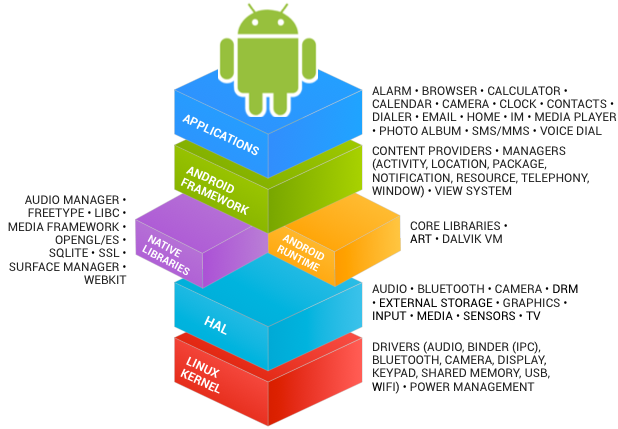
\includegraphics[width=1.0\textwidth,height=10cm]{2}
	\citep{androiddiagram}
	\caption{Android OS Architecture}
	\label{2}
\end{figure}
\section{Processes in Linux and Android}
\subsection{What is a Process?}


A process is a program in execution and is meant to carry out tasks within the operating system. A process is a run time volatile entity created by the system call exec().

\subsection{Difference between Program and Process}

We cannot use \textit{Process} and \textit{Program} interchangeably. A  program is a file containing algorithm expressed in some suitable programming language or notation. It does not execute and just resides on the disk. Hence, it is a passive entity. Whereas a  process has a lifecycle. It is born, runs for some time and then dies and hence it is an \textit{active} entity. A program can be executed by multiple persons, each running a copy of the same program file, but each person is executing a different process. It can be said that a program is only a part of a process.  

\subsection{Properties of a Process}

A process may be created by other processes through system calls like fork or spawn. The process which creates a process is the \textit{Parent} process and the process created is called the \textit{Child} process. Every process will have a parent process except the very first process created: \textit{init}. The parent process is expected to outlive the child process. Every process will be identified using the process identifier \textit{PID}. It is assigned to the process by the OS. Usually, it will be 1+ the last born process pid. The parent PID will also be associated with a process. The PID of init process is 1. Every process has an owner.

A process will use many system resources, during its lifetime. It will use the CPU to run its instructions and the system\textquotesingle s physical memory to hold its data. It will open, access, modify or create files within the filesystems and may directly or indirectly use other physical devices or resources in the system. 

\subsection{Process in Memory}
Process memory has four sections.
\begin{itemize}
	\item The text section has the compiled program code, read from the non-volatile storage when the program is launched.
	\item The data section has global and static variables which are allocated and initialized prior to executing main.
	\item The heap is for dynamic memory allocation and is managed via calls to new, malloc, free, delete, etc.
	\item The stack is used for local variables. The space in the stack is freed when the variables go out of scope. 
\end{itemize}        
When processes are swapped out of memory and later restored, additional information must also be stored and restored. Important among them are the program counter and the value of all program registers.



\subsection{Process Control Block}
For every process, there is a Process Control Block, PCB, which stores the following details.

\begin{itemize}
	\item    Process State - State of the process such as running, waiting,.
	\item    Process ID, and parent process ID.
	\item    CPU registers and Program Counter - They are saved and restored when swapping processes in and out of the CPU.
	\item    CPU-Scheduling information - Contains information like priority information and pointers to scheduling queues.
	\item    Memory-Management information - Contains page tables or segment tables.
	\item    Accounting information - time consumed by kernel CPU, account numbers, limits, etc.
	\item    I/O Status information - Devices allocated for this process, opened file tables, etc.
\end{itemize}


\subsection{Process Vs Threads}
\begin{itemize}
	\item  Processes are disjoint from each other. Their address spaces are disjoint. They are unaware of each other. OS schedules their execution.
	\item  A thread is part of a process. Several threads share a process and the address space is overlapping. The language (eg., C, JAVA) runtime schedules the execution. 
\end{itemize}

\subsection{Process States}
Each process may be in any one of the five states mentioned below.
\begin{itemize}
	\item New       - The process is in the initial stage of being created.
	\item Ready     - The process has all the resource available and is ready to execute, but the CPU is not working on the instructions of this process.
	\item Running   - The CPU is working on the instructions of this process.
	\item Waiting   - This process is not running at the moment, as it is waiting for some other resources for its job.  For example, it may wait for a keyboard input, interprocess message or for a child process to finish.
	\item Terminated- The process has completed.  
\end{itemize}

\begin{figure}
	\centering
	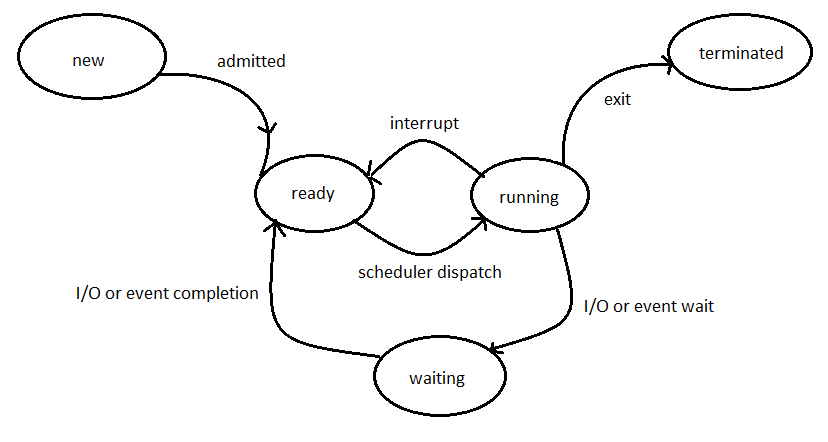
\includegraphics[width=1.0\textwidth,width=15cm,height=7cm]{process_states.png}
	\caption{Process States}
\end{figure}

\subsection{Processes in Android}
In Android, each application gets a unique Linux user ID. 
The system sets permissions for all the files in 
an application so that only the user ID 
assigned to that application can access them.
Each process has its own Dalvik/Art VM.
Every application runs in its own Linux 
process. A process can have multiple threads.


In Android, all components of  an application run in the same process. But if we want to change which process a certain component belongs to, we can change this in the manifest file. 


The manifest entry for component elements  -  Activity, Service, Receiver, and Provider supports an android:process attribute that can specify a process in which that component should run.  We can also set android:process such that components of different applications run in the same process, provided that the applications should have the same Linux user ID and must be signed with the same certificates.


In Android, application process\textquotesingle s lifetime  is not controlled by the application itself. It is determined by the memory available in the system, parts of the application and the importance of the things to the user.


Android determines which process to be killed, when the memory is low, based on importance hierarchy. This hierarchy is formed based on the components running in them and the state of  the components. The classification of process types, based on importance hierarchy are listed in the order of importance.

\begin{itemize}
	\item Foreground Process - A process that is required for what the user is doing, currently.
	\item Visible Process - This is holding an \textit{Activity} that is visible to user, but it is not in the foreground.
	\item Service Process - A process that is holding a \textit{Service} that started with startService() method. Background MP3 plaayback is an example of Service Process.
	\item Background Process - This holds an \textit{Activity} component that is not currently visible to the user.
	\item Empty Process - This process does not hold an active application component.
	
	It is clear that application components play a major role in determining the lifetime of an application process.
	
\end{itemize}
\subsection{Applications and Task}
Android applications are run by processes and their included threads.  The two
terms task and application are linked together tightly, given that a task can be seen
as an application by the user.  In fact tasks are a series of activities of possibly
multiple applications.  Tasks basically are a logical history of user actions, e.g.
the user opens a mail application in which he opens a specific mail with a link
included which is opened in a browser. In this scenario the task would include two
applications (mail and browser) whereat there are also two
Activity
components of
the mail application and one from the browser included in the task. An advantage
of the task concept is the opportunity to allow the user to go back step by step like
a pop operation on a stack.
\subsection{Native Process Vs Android Application}
\begin{itemize}
	\item Application - An application is a software that is designed to help the user to do a specific task. It interacts with the user.
	\item Process - A program contains code for performing tasks, what an application requires. A process is a program in execution. An application accomplishes its task by using processes.  
\end{itemize}

\subsection{Components in Android Lifecycle}

The most important components of the Android application are
\begin{itemize}


\item Activity - 

    represents a user interface screen, window or form;
    an Android application can have one or more activities; an agenda application can have an activity to manage contacts, an activity to manage meetings and one to edit an agenda entry;
    each Activity has its own lifecycle independent from the application process lifecycle;
    each Activity has its own state and it is possible to save it and restore it;
    activities can be started by different applications (if it is allowed);
    has a complex lifecycle because applications can have multiple activities and only one is in the foreground; using the Activity Manager, the Android System manages a stack of activities which are in different states (starting, running, paused, stopped, destroyed);
    in the Android SDK is implemented using a subclass of Activity class which extends the Context class;

\item Intent - represents an entity used to describe an operation to be executed; is a message transmitted to another component in order to announce an operation;
    somehow similar to the event-handler concept from .NET or Java;
    an asynchronous message used to activate activities, services and broadcast receivers;
    implemented by the Intent class;

\item Service - a task that runs in the background without the user direct interaction;
    implemented by a subclass of Service;

\item Content provider - a custom API used to manage application private data;
    a data management alternative to the file system, the SQLite database or any other persistent storage location;
    implemented as a subclass of ContentProvider;
    a solution to share and control (with permissions) data transfer between applications (i.e. Android system provides a content provider for the user’s contact information);

\item Broadcast receiver - a component that responds to system-wide broadcast announcements;
    somehow similar to the global (or system event) handler concept;
    implemented as a subclass of BroadcastReceiver.

\end{itemize}

\subsection{Current Process and Past Process}

This thesis works on the details of the present and past process. We discussed the different states of a process in the previous section. The process in running state is termed as present or current process. The process which was running and got terminated is termed as the past process.

\section{/procfs file system}


/proc file system is a virtual file system in Unix which acts as a window to the Linux OS. This file system does not exist on disk, but the kernel creates it in memory. So this is also called a pseudo filesystem. ls -l shows size as zero and also file command gives the output /textit{empty} as the files are generated instantly when these files are accessed. 


It contains all the information regarding the processes and other system information. There are process specific and Kernel specific entries within this filesystem. The mount point of this file system is called /proc. This is mounted at boot time. 
Many of the system utilities are read
calls to the files in /proc. For example, lsmod is equivalent to cat /proc/modules. Another example is the free command, which reads the memory information from /proc/meminfo file, formats it, and displays it. This file system is also used to change certain kernel parameters at run time.
sysctl is a utility used to change kernel parameter. It  
is
equivalent to altering the files in
/proc/sys, which has all the configurable
kernel parameters as files that are writable. By altering the files located under /proc directory we can alter the kernel parameters in runtime.

There are two types of folders within this directory - numbered and unnumbered. The numbered folders correspond to the pids of all the running processes. Each running process has a folder inside this directory namely /proc/PID, where PID is the process id. Many details regarding the process can be obtained from files within /proc/PID


\subsection{Numbered Files within /proc directory}

Some of the important files within a numbered directory are 
\begin{itemize}
	\item   cmdline - command line of the command.
	\item   environ - environment variables.
	\item   fd - Contains the file descriptors which are linked to the appropriate files.
	\item  limits - Contain the information about the specific limits to the process.
	\item mounts - mount related information
	\item stat - Process status
	\item status - Process status in human readable form
	\item statm - Process memory status information
\end{itemize}
Following are the important links under each numbered directory (for each process).

\begin{itemize}
	\item cwd - Link to the current working directory of the process.
	\item exe - Link to the executable of the process.
	\item root - Link to the root directory of the process.
\end{itemize}
\subsection{Files in /proc directory}

\begin{itemize}
	\item /proc/cpuinfo - information about CPU.
	\item /proc/meminfo - information about memory.
	\item /proc/loadvg  - load average.
	\item /proc/partitions - partition related information.
	\item /proc/version - Linux version.
\end{itemize}
\subsection{Sysfs File System}

Sysfs is a virtual filesystem  similar to /proc. It is exported by the Kernel. It was introduced in Linux 2.6 Kernel. The files within Sysfs contain details about devices and drivers. This file system enables to view the device topology of a system as a simple file system. Some files in this file volume are writable, for configuration and control of devices attached to the system. The mount point for Sysfs is on /sys. It is the union of proc, devfs and devpty file system. This file system lists the devices and buses attached to the system into a file system hierarchy that can be accessed from user space. It is designed in a structured way to handle the device and driver specific options that have previously resided in /proc/, and contain the dynamic device addition previously offered by devfs.

There are seven sub-directories within  sysfs are block, bus, class, devices, firmware, module, and power. 
\begin{itemize}
	\item The /block/ directory   - It contains one directory for each of the registered block devices on the system. 
	\item The /bus/ directory     -It provides a view of the system buses. 
	\item The /class/ directory   - It contains directories that group together similar devices such as network devices, SCSI tape drives, ttys and other miscellaneous devices.
	\item The /devices/ directory  - It provides a  view of the device topology of the system. It has the hierarchy of device structures inside the kernel.
	\item The /firmware/ directory - It contains a system-specific tree of low-level subsystems such as ACPI, EDD, EFI, and so on. 
	\item The /power/ directory          - It contains system-wide power management data.
\end{itemize}

\section{System Calls in Linux}

System calls are methods called by an application to request a service from the Operating System. The primary aim of an Operating System is to provide Process Management, File Management, Memory Management and other things like timing, scheduling and network management. An application uses the required System Call to perform the service it requires. Hence, they are said to be an interface between the application and Operating System Kernel. There are over 300 system calls in Linux.


\subsection{System Calls Related with Process Management}
\begin{itemize}
	\item fork()       - Creates a child process identical to parent 
	\item waitpid()    - Wait for a child to terminate
	\item s=execve()   - Executes the program pointed to by filename.
	\item exit(status) - Terminate process execution and return status   
	
\end{itemize}

\subsection{File Management Related System Calls}
\begin{itemize}
	\item fd=open(file, how,.)                Open a file for reading, writing or both.
	\item s=close(fd)                        Close an open file
	\item n = read(fd, buffer, nbytes)         Read data from a file to a buffer
	\item n = write(fd, buffer, nbytes)        Write data from buffer to a file
	\item position = lseek(fd, offset, whence) Move the file pointer 
	\item s = stat(name,\&buff)              Get a file\textquotesingle s status information
\end{itemize}
\subsection{Network Connection Related System Calls}
\begin{itemize}
	
	\item socket          - Creates a socket.
	\item connect         - This system call is used to connect referred to by the file descriptor to the addr specified
	
	\item bind            - Assigns a local protocol address to a socket
	\item listen          - Listens for connections on the socket 
	\item accept          - This is called by the TCP server to return the next completed
	connection from the front of the completed connection queue.
	\item recvfrom         - Receives a message from a socket.  	                        
	\item close           - Marks the socket as closed and returns to the process
	immediately.                         
\end{itemize}
\section{Strace}

Strace is a tool used to trace the system calls and signals used by a process. It is a useful diagnostic and debugging tool. It intercepts and records the system calls called by a process and the signals received by a process. The system call\textquotesingle s name, its arguments, and its 
return value are printed to stdout or to the file specified with 
the -o option. 

\subsection{Options}

Here are some of the important options to be used with Strace

\begin{table}[H]
	\centering
	\caption{Options to be used with Strace}
	\label{strace-options}
\begin{tabular}{|l|l|}
	\hline
	Options          & \multicolumn{1}{c|}{Description}                                                                                                                                             \\ \hline
	-h               & \begin{tabular}[c]{@{}l@{}}Trace child processes as they are created by currently\\  traced processes as a result of the fork(2) system call.\end{tabular}                   \\ \hline
	-o filename      & \begin{tabular}[c]{@{}l@{}}Write the trace output to the file filename rather than\\ to stderr.\end{tabular}                                                                 \\ \hline
	-p pid           & \begin{tabular}[c]{@{}l@{}}Attach to the process with the process ID pid and \\ begin tracing.\end{tabular}                                                                  \\ \hline
	-e expr          & \begin{tabular}[c]{@{}l@{}}A qualifying expression which modifies which events to trace or \\ how to trace them.\end{tabular}                                                \\ \hline
	-e trace=set     & Trace only the specified set of system calls.                                                                                                                                \\ \hline
	-e trace=file    & Trace all system calls which take a file name as an argument.                                                                                                                \\ \hline
	-e trace=process & \begin{tabular}[c]{@{}l@{}}Trace all system calls which involve process management. \\ This is useful for watching the fork, wait, and exec steps of a process.\end{tabular} \\ \hline
	-e trace=network & Trace all the network related system calls.                                                                                                                                  \\ \hline
	-tt              & Prefix each line of the trace with time in microseconds                                                                                                                      \\ \hline
	-s strsize       & Specify the maximum string size to print (the default is 32).                                                                                                                \\ \hline
	-v               & Print unabbreviated versions of environment, stat, termios, etc. calls.                                                                                                      \\ \hline
	-T               & \begin{tabular}[c]{@{}l@{}}Show the time spent in system calls. This records the time difference \\ between the beginning and the end of each system call.\end{tabular}      \\ \hline
\end{tabular}
\end{table}


\subsection{Some Problems in Strace}
\begin{itemize}
	\item Strace interferes with process flow
	
	The use of strace with a process causes additional computational overhead and many contexts
	switch between the program and
	strace. When system performance is a priority, we should be careful in using Strace.
	
	
	\item Strace Output Readable to All Users
	
	The output of strace is in a readable format to all users. It may disclose some sensitive information. For example, it may display the private SSH key in read() while tracing the execution of SSH. 
\end{itemize}


\section{ltrace}
\begin{itemize}
	\item ltrace can be used to trace shared library calls. This can be very useful to get
	insight into the program 
    \item It is an useful debugging and reverse engineering tool.
    \item Programs use system calls to access system resources such as opening a file or connecting to the network. Library calls are calls made to the GNU C library which provides a more programmer-friendly interface to the system.
    \item This tool is very useful for debugging user-space applications to determine which library call is failing. It is also capable of receiving signals for segmentation faults, etc.
    
\end{itemize}
\subsection{Debugging a program with ltrace}	
	
	\begin{lstlisting}
           1.  #include <stdio.h>
           2.  #include <unistd.h>
           3.            
           4.  int main()
           5.  {
           6.    FILE *fp = fopen("rfile.txt", "w+");
           7.     fprintf(fp+1, "Invalid Write\n");
           8.     fclose(fp);
           9.     return 0;
           10. }
	\end{lstlisting}
	
	When we compile and run this program 
	\begin{lstlisting}
	        anusuya@ubuntu:~/source$ gcc file.c -Wall -o file
	        anusuya@ubuntu:~/source$./file
	        Segmentation fault (core dumped)
	\end{lstlisting}
	
	We can ltrace to debug this code and find the details of error
	
	\begin{lstlisting}
	         anusuya@ubuntu:~/source$ltrace ./file
	         __libc_start_main(0x8048454, 1, 0xbfc19db4, 0x80484c0, 0x8048530 <unfinished ...>
	         fopen("rfile.txt", "w+")                          = 0x9160008
	         fwrite("Invalid Write\n", 1, 14, 0x916009c <unfinished ...>
	         --- SIGSEGV (Segmentation fault) ---
	         +++ killed by SIGSEGV +++content...
	\end{lstlisting}
	
	The first line states the libc function call main(), with its parameters and it terminated unfinished. Since we saw the segmentation fault, so unfinished main() aligns with our understanding.
	
	Next line has listed the fopen() call to open rfile.txt in write plus mode and returning a valid file pointer address. 
	Moving on to the next library call, we have fwrite which is unfinished. Here is the bug because of which program crashed. So focusing on this call and analyzing, notice the file pointer containing the address in fwrite() call doesnt match the one in fopen() call. Hence, the crash. The program is trying to write onto a file using file pointer which is invalid following a SIGSEGV signal.
	Getting back to our program, the bug is in line 7 of our program where the file pointer being passed to the fprintf() call is tampered. So, we just found the bug.

    \begin{lstlisting}
             fprintf(fp, "Invalid Write\n");
    \end{lstlisting}
    
\section{Strace and ltrace comparision}
The advantage of strace over ltrace is that the information is often simpler. Not all library calls map to system calls. The disadvantage is that not all library calls have the same name as their system call equivalent. For example, the fork() library call uses the clone() system call which can also be used for threading as well as making a new process.
ltrace only traces calls from the executable to the 
libraries the executable is linked against. It does not trace calls between libraries.
Hence, calls such as to the printf() function (which itself resides in the libc shared library) is not shown. Also, there is no option to include the library name in the output for each of the
called functions. But we can still trace scripts by tracing the script interpreter.

\begin{lstlisting}
         ltrace python myscript.py
\end{lstlisting}

\begin{figure}[H]
	\centering
	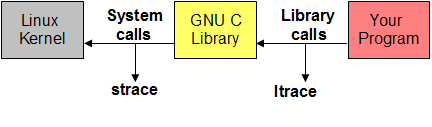
\includegraphics[width=1.0\textwidth,width=10cm,height=5cm]{lib_sys_calls}
	\caption{ltrace and strace}
\end{figure}
\section{Cloud Upload}

This thesis is going to generate a lot of log files as a part of using tools like strace and ltrace. It is difficult to store and manage a large number of files on a local disk. So we prefer to use cloud storage, a method of storing our digital data in logical pools where the physical storage spans across  multiple servers and locations and the physical environment are owned and managed by a hosting company, usually called Cloud Storage Providers. The cloud storage providers are responsible for keeping the data available and accessible, and the physical environment protected and running. People and organizations buy or lease storage capacity from the providers to store user, organization, or application data.

Cloud storage can provide the benefits of greater accessibility and reliability, rapid deployment, strong protection for data backup, archival and disaster recovery purposes, and lower overall storage costs as a result of not having to purchase, manage and maintain expensive hardware. There are many benefits of using cloud storage, however, cloud storage does have the potential for security and compliance concerns that are not associated with traditional storage systems.

\subsection{Types Of Cloud Storage}
\begin{itemize}
	\item Personal/Mobile Cloud Storage
	It is used for storing individual\textquotesingle s data in the cloud. The person will be given access to the data from anywhere. It can be used to backup data in the mobile device. It is subset of Public Cloud Storage.
	
	\item Public Cloud Storage
	This is used by enterprises where they have rented or subscribed for the cloud storage for a certain period of time. The cloud server is fully managed by the cloud storage provider. Anyone with valid access and user credentials can access the data from anywhere in the world. 
	
	\item Private Cloud Storage
	This type is used by an individual or a company. The cloud storage provider sets up the data center in the user\textquotesingle s space or premise. This provides more security and restricted access to data.
	\item Hybrid Cloud Storage
	This is a combination of public and private cloud storage. Here some data is stored in public cloud storage. Sensitive data is stored using private cloud storage, in the user\textquotesingle s place and has restricted access.
	
	We will be using the personal cloud storage for our thesis. 
\end{itemize}
\chapter{Provenance of a Process}
	
	\section{Provenance of a Process}
	        The word \textit{provenance} means origin, source or history of ownership of an object.
		Provenance of a process means getting the details of its origin, source and also what all it does during its lifetime.
                By knowing the provenance of a process, we will be able to tell the time of creation of the process, by which process it was triggered, what are all the child processes it invoked, it activities during its life period and also the time it ended
		It should also provide all the details of files it opened, created, written and also the network connections it spawned.
	
	\section{Method}
	The provenance of a process is obtained by analysing the system calls and library calls a process used while execution.
	
	Monitoring Linux utility tools like strace and ltrace are used to monitor and record the system calls and library calls a process used.
  
    These tools are attached to all the running process. 
    The output obtained using these tools are logged. The logged details are then analysed.
    
    Program for running the strace and ptrace tools is written in a script.
	
	This script should be always up and running, whenever the device is booted.
	
	\subsection{Past Process}
	Whenever a process gets terminated, the output of the strace and ltrace are sent to a log file. The log files are interpreted to get the provenance of a process.
	
	\subsection{Current Process}
	The details of current processes can be gathered from the /proc directory. So we have to define an API such that it reads the files within /proc directory and displays the details.
	
	We can use JNI(Java Native Interface) or Android API\textquotesingle s like ApplicationInfo, ActivityManager.
	
	
	
    \begin{figure}
    	\centering
    	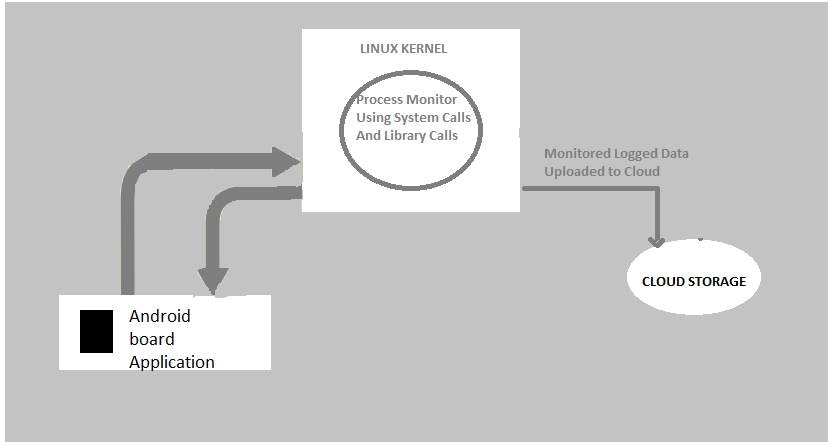
\includegraphics[width=1.0\textwidth,width=15cm,height=11cm]{Archi_jul11}
    	\caption{Architecture Of the System}
    \end{figure}
\chapter{Problem Solution Architecture}

This section describes solutions to various problems that evolved while developing and implementing the thesis.

\section{Strace in Android}
Strace is not a built in tool in Android. So we have to install it in Android. The Android device must be rooted for installing strace. The following steps explains how to install strace in Android.
\begin{itemize}
	\item Download the strace source distribution from the SourceForge strace project
	\item Extract the strace package on your linux machine.
	\item Set your compiler information:
    \begin{lstlisting}
           export CC=your_cross_compiler_folder/bin/arm-none-linux-gnueabi-gcc
           export STRIP=your_cross_compiler_folder/bin/arm-none-linux-gnueabi-strip
           export CFLAGS="-O2 -static"
    \end{lstlisting}
    
    \item Add cross\_compiler folder /bin into your \$PATH.
     \item Change your current folder to the strace folder (where you extracted the source), use command.
     
     \begin{lstlisting}
        ./configure --host=arm-linux
     \end{lstlisting}
     
    \item Compile
    \begin{lstlisting}
        make
    \end{lstlisting}
    \item Verify result
	\begin{lstlisting}
	   file strace
	\end{lstlisting}
	The output would be like
	\begin{lstlisting}
	  strace: ELF 32-bit LSB executable, ARM, version 1 (SYSV), for GNU/Linux 2.6.14, statically linked, not stripped
	\end{lstlisting}
\end{itemize}

\section{Filtering Strace Output}
	The output of
	strace
	can quickly become very large and synchronous output to
	strerr
	or a log file may
	greatly impair program performance. If we know up front which system calls are of importance, we
	may limit the output to one or a few kernel calls (or e.g. with
	-e file
	system calls with file names). This
	slows down program execution considerably less and makes subsequent evaluation of the
	strace	output	much easier. For our thesis, we concentrate mostly on file and network related system calls.
	
\section{Disadvantages Of Using JNI}
\begin{itemize}
	\item Bad C/C++ code in native library will cause core dumps / segmentation faults that the JVM cannot recover from. This may result in crashing of the whole app.
	\item Difficult to debug runtime error in native code.
	\item Potential security risk.
\end{itemize}

\section{Storage}
A cloud storage for the collected log files is preferred, as the log files keeps on getting accumulated while the processes are running.

All the logged details will be uploaded in cloud server. A log uploader will be uploading all the logs to clouds in a configurable way like configurable time interval for log upload. All the uploaded logs will be deleted from the device.

JSON and OAuth API is used for cloud integration. There are many free cloud storage providers available. We can choose any one of them, for our cloud upload.

\chapter{Implementation and Results}

\section{APK Created}
We created an application named \textit{ANU DASHBOARD OF PAST AND PRESENT PROCESS}. This has various 5 tabs - Past Process, Basic Info, Application, Process and Net Stats.

 \begin{figure}[H]
	\centering
	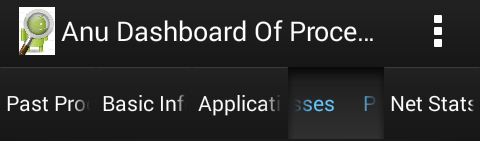
\includegraphics[width=1.0\textwidth,width=10cm,height=2cm]{tabs}
\end{figure} 

The tabs
\begin{itemize}
	\item Past process has process name, process id, time started, time ended, files opened, files written, files read, network connection it spawned.
	\item Basic Info has details of internal storage, sd card storage, battery, memory, processor.
	\item Application Info has details of all the running application, its package name, user id, install date, file size.
	\item Process has details of running processes, process id, user id, state, importance, lru
	\item Net stats - It displays the network details, local/remote address, state.
\end{itemize} 

A shell script is created to get the strace of all the running process and once it terminated, it will be stored in a text file, with the timestamp appended to the name.

\subsection{Past Process}
In the past process tab, the list of all the past processes name are listed based in a chronoligaical order. We can select the time from when the past processes should be listed - last one hour, last one day and last one week.
\begin{figure}[H]
	\centering
	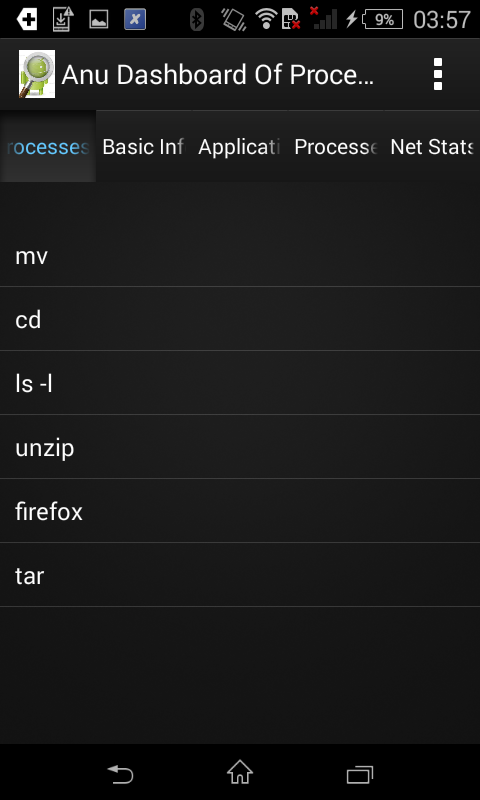
\includegraphics[width=1.0\textwidth,width=5cm,height=7cm]{past_process_list}
	\caption{List of Past Processes}
	\end{figure}
	When we click on each past process, we get the details like pid, time started, time ended, files opened, files written, network connection it used. 
	\begin{figure}[H]
		\centering
		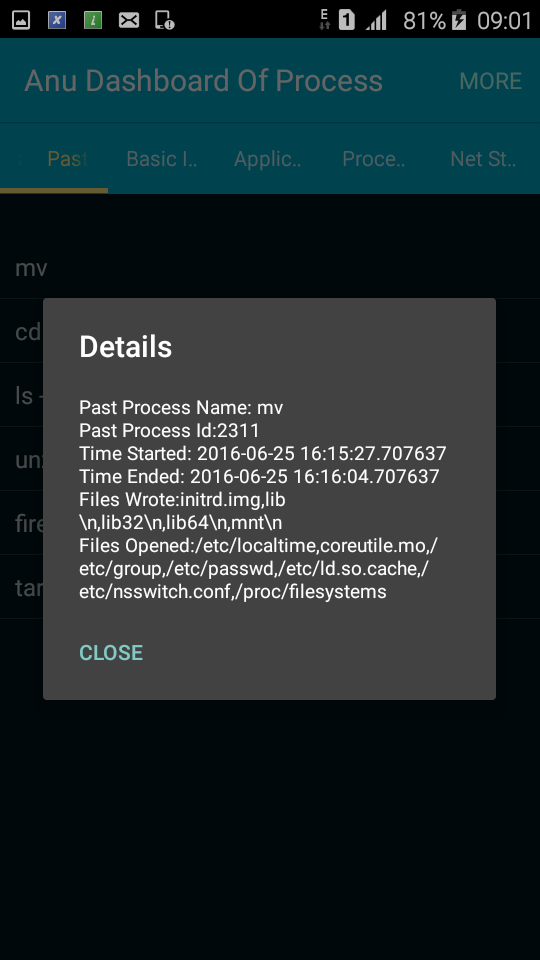
\includegraphics[width=1.0\textwidth,width=5cm,height=7cm]{past}
		\caption{Details of Past Processes}
	\end{figure}
\subsection{Basic Info}
In the basic info tab details like battery, SD card storage, A2SD storage, internal storage, system storage, system cache, processor and memory are listed.
 
\begin{figure}[H]
	\centering
	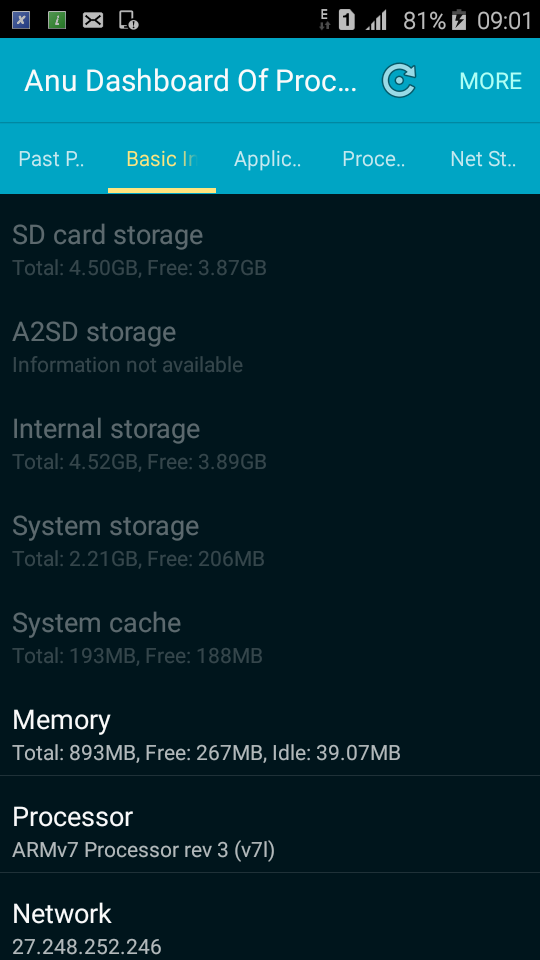
\includegraphics[width=1.0\textwidth,width=5cm,height=7cm]{storage}
	\caption{Storage}
\end{figure}
When we click on the battery item, we get details like level, health, status, technology, voltage, temperature, plugged.
\begin{figure}[H]
	\centering
	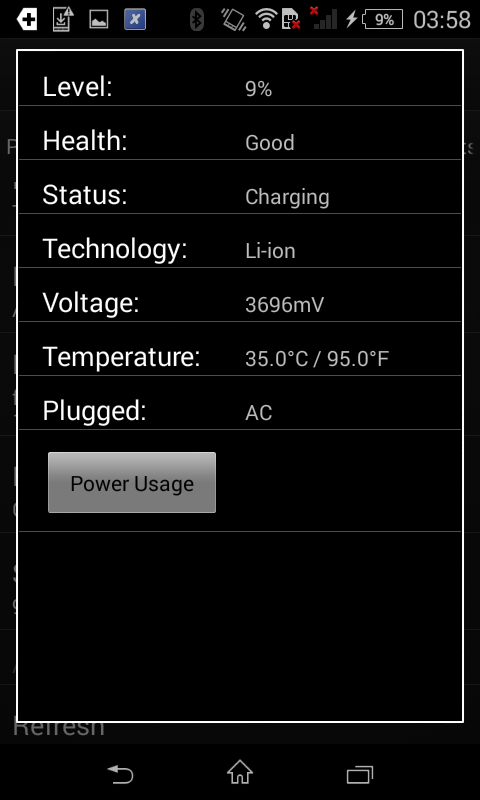
\includegraphics[width=1.0\textwidth,width=5cm,height=7cm]{battery_details}
	\caption{Battery Information}
\end{figure}
When we click on the processor, we get details like model, current frequency, cpu frequency range and scaling governor.
\begin{figure}[H]
	\centering
	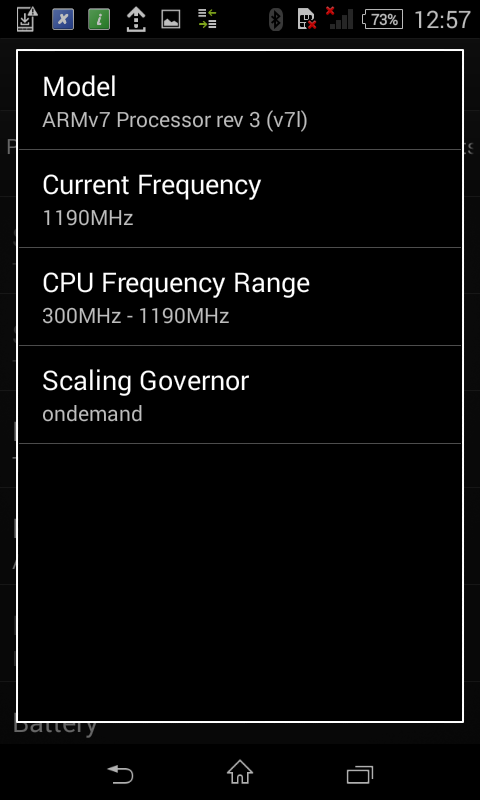
\includegraphics[width=1.0\textwidth,width=5cm,height=7cm]{processor_details}
	\caption{Processor Details}
\end{figure}
\subsection{Application}
Under the \textit{Application} tab, all the current running applications are listed.
\begin{figure}[H]
	\centering
	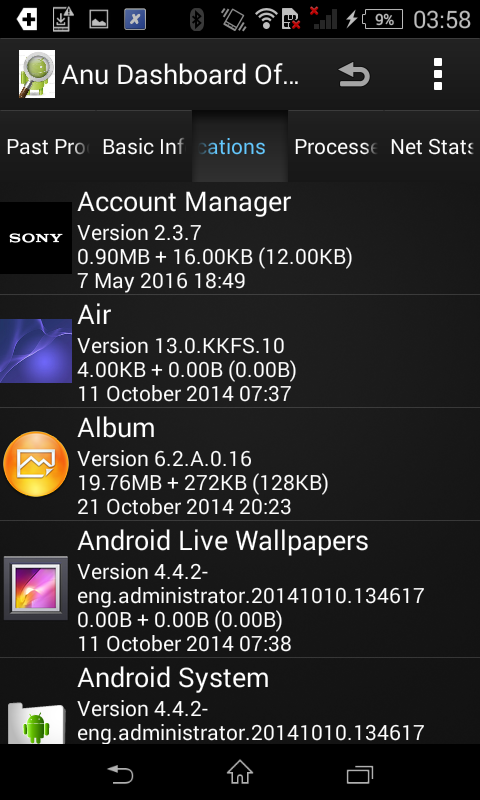
\includegraphics[width=1.0\textwidth,width=5cm,height=7cm]{application_list}
	\caption{All The Running Application}
\end{figure}
When we click on each application, we get details like package name, user id, file size, public source, install date, permission, flags and enabled.
\begin{figure}[H]
	\centering
	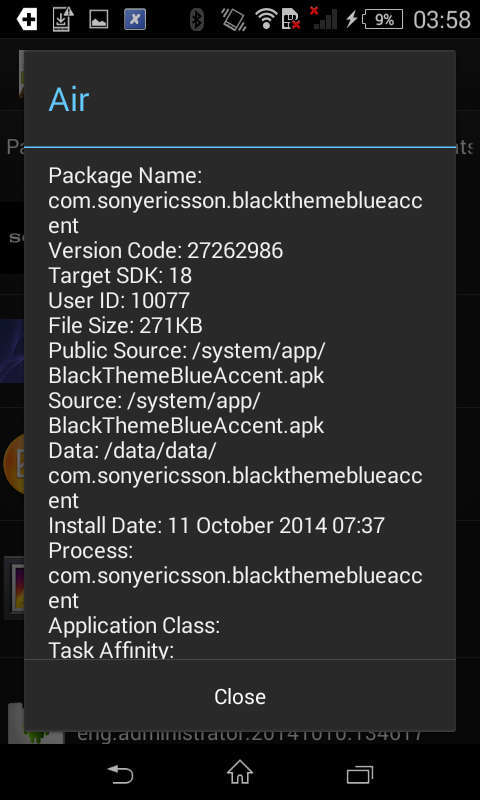
\includegraphics[width=1.0\textwidth,width=5cm,height=7cm]{application_details}
	\caption{Details Retrieved Of An Application}
\end{figure}
\subsection{Processes}
Under the \textit{Processes} tab, all the current processes are displayed. Color differentiation is given for different type of processes like - foreground process(blue), background process(yellow), system services(grey).
\begin{figure}[H]
	\centering
	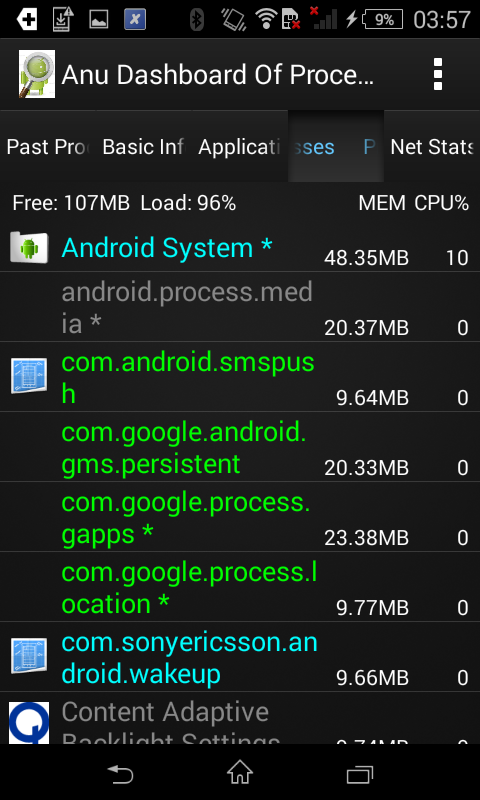
\includegraphics[width=1.0\textwidth,width=5cm,height=7cm]{Process_list}
	\caption{Process List}
\end{figure}
\begin{figure}[H]
	\centering
	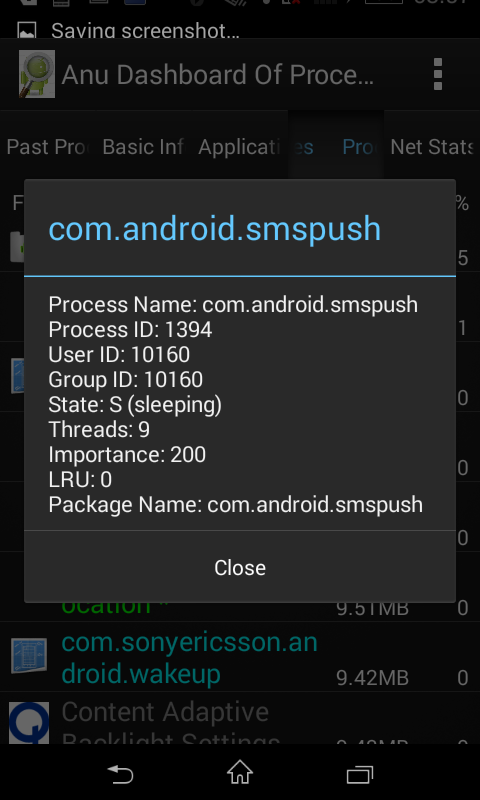
\includegraphics[width=1.0\textwidth,width=5cm,height=7cm]{process_details}
	\caption{Process Details}
\end{figure}
When we click on each process, we get details like process name, process id, user id, group id, state(sleeping, runnin,.), threads, importance, lru, package name.
\subsection{Net Stats}
Under \textit{Net Stats}, we get the details of the protocol used, local/remote address, state of the protocol.
\begin{figure}[H]
	\centering
	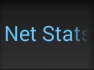
\includegraphics[width=1.0\textwidth,width=5cm,height=7cm]{network_details}
	\caption{Network State}
\end{figure}
The current network type, local address, roaming state, ip address are displayed.
\begin{figure}[H]
	\centering
	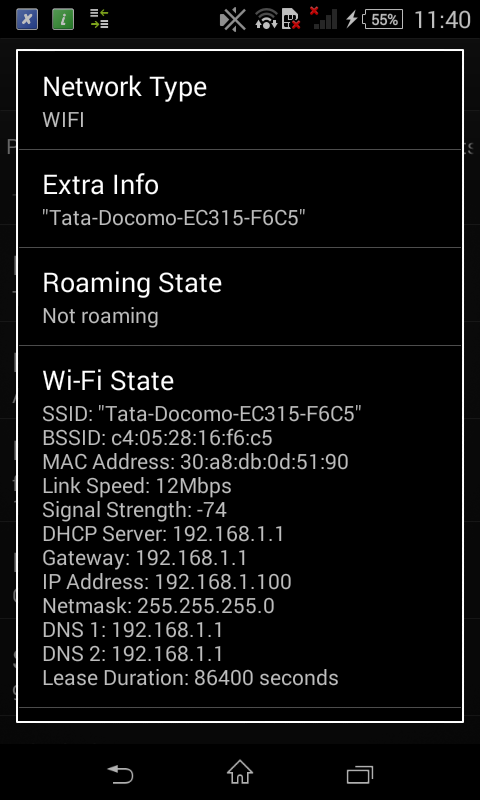
\includegraphics[width=1.0\textwidth,width=5cm,height=7cm]{nw_connection_details}
	\caption{Network Connection}
\end{figure}


\section{Details of the APK}

The stastistics of the sourcecode obtained using cloc is given in the Table \ref{source-code}

\begin{table}[H]
	\centering
	\caption{Source Code Statistics}
	\label{source-code}
	\begin{tabular}{lllll}
		\hline
		\multicolumn{5}{c}{http://cloc.sourceforge.net} \\ \hline
		Language  & Files  & Blank  & Comment  & Code   \\ \hline
		JAVA      & 16     & 3118   & 699      & 14391  \\ \hline
		XML       & 25     & 68     & 1        & 813    \\ \hline
	\end{tabular}
\end{table}


\section{Link to source code}

The source code of the project is available in the following link.
http://www.github.com/anurp/AnuDashboardOfProcess

Related app to this thesis, OSMonitor source code are available in the link

http://www.github.com/anurp/OSMonitor
\chapter{Methods Used}


\section{Running Process Details}
As we discussed the disadvantages of JNI, in the previous chapter, we are using Android classes and methods to get the information of processes and all the device and OS related information.

We want to list all the currently running processes with all the details. This can be achieved with the class ActivityManager.RunningAppProcessInfo.

To get the process name.
\begin{lstlisting}

        String procName = rap.procInfo.processName;
\end{lstlisting}


Process ID:

\begin{lstlisting}

        int procId = procInfo.pid;
\end{lstlisting}

To List The Processes Based On IMPORTANCE:

We have five fields to determine the importance of a process


\begin{lstlisting}


        RunningAppProcessInfo.IMPORTANCE_FOREGROUND; 

        RunningAppProcessInfo.IMPORTANCE_PERCEPTIBLE; 
       
        RunningAppProcessInfo.IMPORTANCE_VISIBLE; 

        RunningAppProcessInfo.IMPORTANCE_SERVICE; 
       
        RunningAppProcessInfo.IMPORTANCE_BACKGROUND; 

        RunningAppProcessInfo.IMPORTANCE_EMPTY; 

\end{lstlisting}

lru:

\begin{lstlisting}
        procInfo.lru
\end{lstlisting}


\section{Retrieving Application Details}
Android Application is the software running in the device. To get the all the details related to Android running Applications, we can use the class ApplicationInfo. 

To list all the Applications:
\begin{lstlisting}

        final List<ApplicationInfo> filteredApps = filterApps( allApps );
\end{lstlisting}

To get the Package name of the Application:

\begin{lstlisting}


        String pkgName = ai.appInfo.packageName;
\end{lstlisting}

\section{Retrieving Network Connection Related Information}

Network Connection Related Information can be obtained from class ConnectivityManager;

This class answers queries about the state of network connectivity. It also notifies applications when network connectivity changes. Get an instance of this class by calling
\begin{lstlisting}

         Context.getSystemService(Context.CONNECTIVITY_SERVICE).
\end{lstlisting}
The primary responsibilities of this class are to

\begin{itemize}

 	\item    Monitor network connections (Wi-Fi, GPRS, UMTS, etc.).
    \item Send broadcast intents when network connectivity changes.
    \item Attempt to fail over to another network when connectivity to a network is lost.
    \item Provide an API that allows applications to query the coarse-grained or fine-grained state of the available networks.
    \item Provide an API that allows applications to request and select networks for their data traffic.
\end{itemize}
We use the method  getActiveNetwork() of this class to the network connection details like Network Type, Roaming State and Extra Info.

Returns a Network object corresponding to the currently active default data network. 

The class WifiManager provides the primary API for managing all aspects of Wi-Fi connectivity. Get an instance of this class by calling
\begin{lstlisting}


         Context.getSystemService(Context.WIFI_SERVICE). 
         \end{lstlisting}
         It deals with several categories of items.
\begin{itemize}

	\item The list of configured networks. 
	\item The list can be viewed and updated, and attributes of individual entries can be modified.
    \item The currently active Wi-Fi network, if any. 
    \item Connectivity can be established or torn down, and dynamic information about the state of the network can be queried.
    \item Results of access point scans, containing enough information to make decisions about what access point to connect to.
    \item It defines the names of various Intent actions that are broadcast upon any sort of change in Wi-Fi state. 
    \end{itemize}

We use the method getConnectionInfo () to get details such as SSID, BSSID, Mac Address, Link Speed, Signal Strength of wifi connection.

We use the method getDhcpInfo() to get the details such as DHCP server address, gateway address and DNS address.


\section{Battery Information Of The Device}

Battery Manager helps us to retrieve the battery details of the device. The BatteryManager class contains strings and constants used for values in the ACTION BATTERY CHANGED Intent, and provides a method for querying battery and charging properties. 

To know the level of battery.
\begin{lstlisting}

         int level = intent.getIntExtra( "level", 0 ); 
         int scale = intent.getIntExtra( "scale", 100 ); 
         String lStr = String.valueOf( level * 100 / scale ) + '%';
         data.add( new String[]{
         getString( R.string.batt_level ), lStr} );
\end{lstlisting}
To know the health of the battery, whether it is - Good, Over heat, Dead, Over Voltage, Failure.
\begin{lstlisting}
        int health = intent.getIntExtra( "health", BatteryManager.BATTERY_HEALTH_UNKNOWN );
\end{lstlisting}
To know the status of the battery - Charging, Discharging, Full , Not Charging. 
\begin{lstlisting}
        int status = intent.getIntExtra( "status", BatteryManager.BATTERY_STATUS_UNKNOWN );
\end{lstlisting}
To know the temperature of the device.
\begin{lstlisting}
        int temperature = intent.getIntExtra( "temperature", 0 ); 
\end{lstlisting}
To know the voltage of the device
\begin{lstlisting}
        int voltage = intent.getIntExtra( "voltage", 0 ); //$NON-NLS-1$

				String vStr = String.valueOf( voltage ) + "mV"; //$NON-NLS-1$

				data.add( new String[]{
						getString( R.string.batt_voltage ), vStr
				} );
\end{lstlisting}

\section{Cloud Upload Of Log Files}
We use Dropbox to upload our collected log files. We have to use Core API to achieve this. The Core API is based on HTTP and OAuth and provides low-level calls to access and manipulate a user\textquotesingle s Dropbox account. The Core API uses OAuth v2.
A Dropbox account is required for transferring to and from Dropbox Cloud.
We have to register our app in the App console within our Dropbox account. We have to define the app secret and app key while registration.
This will be used in our Android app for upload and download of files.
\begin{lstlisting}
        final static private String APP_KEY = "INSERT_APP_KEY";
        final static private String APP_SECRET = "INSERT_APP_SECRET";
\end{lstlisting}

We have to authenticate our app to the Dropbox. startOAuth2Authentication() method is called to authorize the app.

\begin{lstlisting}
        mDBApi.getSession().startOAuth2Authentication(MyActivity.this);
\end{lstlisting}

More about registering our app in Dropbox and authenticating is explained in details in appendix.
\subsection{Upload Module}

\begin{lstlisting}
        File file = new File("working-draft.txt");
        FileInputStream inputStream = new FileInputStream(file);
        Entry response = mDBApi.putFile("/magnum-opus.txt", inputStream,
                                file.length(), null, null);
        Log.i("DbExampleLog", "The uploaded file's rev is: " + response.rev);

\end{lstlisting}
\subsection{Download Module}
\begin{lstlisting}
        File file = new File("/magnum-opus.txt");
        FileOutputStream outputStream = new FileOutputStream(file);
        DropboxFileInfo info = mDBApi.getFile("/magnum-opus.txt", null, outputStream, null);
        Log.i("DbExampleLog", "The file's rev is: " + info.getMetadata().rev);
\end{lstlisting}

\subsection{Deleting Files After Cloud Upload}
Once the file is uploaded to the cloud, we have to delete the file immediately, to free the space in the device.
There is a java method called mFile.delete(). Once we get the result that theace outp file has been uploaded successfully to the cloud, this method is called and the file gets automatically deleted in the disk. 

\section{Strace for all running processes}
A shell script is used for getting the strace details of all the processes.
\begin{lstlisting}
        #!/usr/bin/env bash
        pid=$(ps ax | perl -nle 'print $1 if /^ *([0-9]+)/')
        for i in "$pid" 
        do
        strace -p $i -o /tmp/strace_$(date).txt  
        done
\end{lstlisting} 

A part of the strace output file obtained is shown below.        .  
\begin{lstlisting}
        2550  16:15:27.707637 execve("/bin/ls", ["ls", "-l"], ["TERM=xterm",        "LS_COLORS=rs=0:di=01;34:ln=01;36:mh=00:pi=40;33:so=01;35:do=01;35:bd=40;33;01:cd=40;33;01:or=40;31;01:su=37;41:sg=30;43:ca=30;41:tw=30;42:ow=34;42:st=37;44:ex=01;32:*.tar=01;31:*.tgz=01;31:*.arj=01;31"...,  "PATH=/usr/local/sbin:/usr/local/bin:/usr/sbin:/usr/bin:/sbin:/bin", "LANG=en_IN", "HOME=/home/anu", "LANGUAGE=en_IN:en", "DISPLAY=:0", "COLORTERM=gnome-terminal", "XAUTHORITY=/home/anu/.Xauthority", "SHELL=/bin/bash", "MAIL=/var/mail/root", "LOGNAME=root", "USER=root", "USERNAME=root", "SUDO_COMMAND=/usr/bin/strace -e fork,read,write,open,close,link,execve,rename,dup,dup2,symlink,clone,vfork,setuid32,setgid32,chmod,fchmod,pipe,truncate,ftruncate,readv,recv,recvfrom,recvmsg,send,sendt"..., "SUDO_USER=anu", "SUDO_UID=1000", "SUDO_GID=1000"]) = 0 <0.000366>
        2550  16:15:27.708604 open("/etc/ld.so.cache", O_RDONLY|O_CLOEXEC) = 3 <0.000031>
        2550  16:15:27.708785 close(3)          = 0 <0.000050>
        2550  16:15:27.708999 open("/lib/x86_64-linux-gnu/libselinux.so.1", O_RDONLY|O_CLOEXEC) = 3 <0.000022>
        2550  16:15:27.709071 read(3, "\177ELF\2\1\1\0\0\0\0\0\0\0\0\0\3\0>\0\1\0\0\0\0[\0\0\0\0\0\0@\0\0\0\0\0\0\0X\5\2\0\0\0\0\0\0\0\0\0@\0008\0\10\0@\0\35\0\34\0\1\0\0\0\5\0\0\0\0\0\0\0\0\0\0\0\0\0\0\0\0\0\0\0\0\0\0\0\0\0\0\0,
        \366\1\0\0\0\0\0,\366\1\0\0\0\0\0\0\0 
     
\end{lstlisting}


\section{Getting The File Related Details From Strace Output}

The system calls related to file management are open, read, write, close. We have to get the file descriptors to retrieve the files that are used while a process is executing. In Open system call, the first argument is the file opened. In Read syscall the first argument is the file descriptor. The file descriptor is the return argument of the Open syscall. 
\begin{lstlisting}


        if (syscall.equals("open")) {
                   
                    String path = args.substring(1, args.lastIndexOf('\"'));
                    String fd = retVal;
        }
        if (syscall.equals("read") || syscall.equals("pread") || syscall.equals("readv") || syscall.equals("recv") || syscall.equals("recvfrom") || syscall.equals("recvmsg")) {
                    String fd = args.substring(0, args.indexOf(','));
        }
\end{lstlisting}


\section{Getting the Network Connection Related Details From Strace Output}
The system calls related to network connection are connect, recv. We get the socket from connect system call.
\begin{lstlisting}

        static final Pattern networkPattern = Pattern.compile("sin_port=htons\\(([0-9]+)\\), sin_addr=inet_addr\\(\"(.*)\"\\)"); 
        
        if (syscall.equals("connect")) {
                    String fd = args.substring(0, args.indexOf(','));
                    String socket = args.substring(args.indexOf('{'), args.indexOf('}') + 1);
        }
        Matcher networkMatcher = networkPattern.matcher(path);
                        if (networkMatcher.find()) {
                            vertex.addAnnotation("subtype", "network");
                            vertex.addAnnotation("address", networkMatcher.group(2));
                            vertex.addAnnotation("port", networkMatcher.group(1));
\end{lstlisting}


\chapter{Related Work}
\section{OS Monitor - A Case Study}


OS Monitor\citep{OSMonitor} is an open source Android app. It is a tool for monitoring our Android system. It displays information such as
\begin{itemize}
	\item Processes - monitor all processes.
	\item Connections - display every network connection.
	\item Misc - monitor battery, processors, network interfaces and file system.
	\item Messages - search dmesg or logcat in real-time.
\end{itemize}
OS Monitor contains two major components, a native executable binary that runs on the background to collect system information, and a user interface.

When UI component sends a request, the background binary will collect and serialize data. The data will be transferred via IPC and renderred on screen. It uses \textquotesingle C \textquotesingle code to read the /proc file directory and Java Native Interface(JNI)

The background binary works in single thread mode, all the requests are queued and processed. 

Communication between Android App and native process is through Unix socket. All requests or responses are serialized by Google flatBuffer.
It also has security features.
OS Monitor is based on Unix socket with a randomized name. Knowing the randomized name, anyone can easily hijack it with his own app. A security token is used to prevent such hijack. Any connection needs to offer a token for validating, otherwise, the connection will be disconnected. 

\begin{figure}
	\centering
	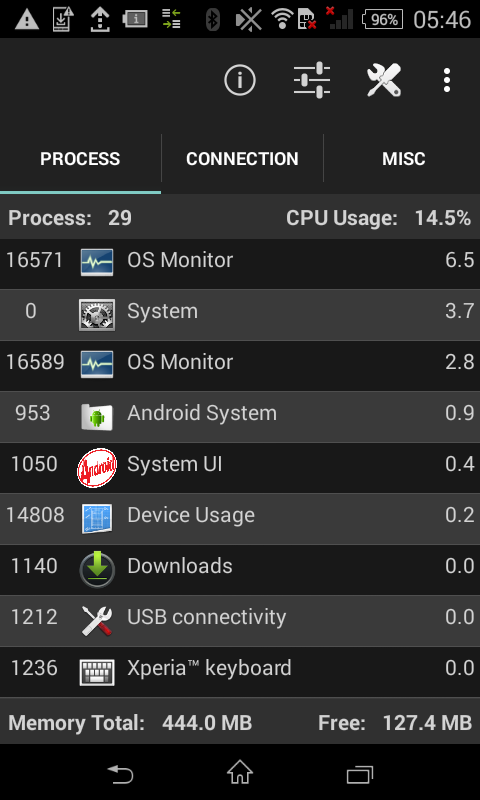
\includegraphics[width=1.0\textwidth,width=5cm,height=7cm]{os_mon.png}
	\caption{Snapshot from OS Monitor app}
\end{figure}
\section{Network Monitoring and Filtering}
Network Ombudsman \citep{Nikhil2015}  is a network monitoring and filtering tool.
It is built in Android  framework.
It categorises and ranks applications as malicious and non-malicious
The Network ombudsman system comprises of a monitoring service, filtering/firewall
service, a log uploader, an android application and a cloud server. 
The monitoring
service will keep tab of all the network connection both internal and external
to the device. The filtering/firewall service will update the rules of the netfilter
system firewall and enables the blocking/unblocking of the devices. This service
will also keep tab of the context changes and reputation changes and changes the
firewall policies accordingly. All the monitored data that will be logged by the
monitoring service will be uploaded into the cloud server by the log uploader.

\section{Process Authentication}

A new process is created when an application or service is launched and the runtime systen becomes the parent process of all user application processes in Android. 
Android has numerous vulnerabilities that leads to failure of application sandboxes.

This Paper \textit{DroidBarrier: Know what is executing on your Android}\citep{almohri2014} uses a technique called \textit{Process  Authentication}  for  Android  applications  to  overcome
the shortcomings of current Android security practices.
A new process is created when an application or service is launched and the runtime systen becomes the parent process of all user application processes in Android. 
Android has numerous vulnerabilities that leads to failure of application sandboxes. For  example, the
Gingerbreak
exploit  affected  the  popular  Android  2.3  enabled  a  malicious  application  to  gain
root
privileges  and
completely  bypass  Android\textquotesingle s  application  sandboxes.
This paper observes that critical vulnerabilities in Android share a root cause: malicious applications that are installed and executed without the user\textquotesingle s consent.
Process
authentication  model  addresses  the  problem  by  regarding
application processes as individuals that must be authenticated  before  using  system  resources. In  this  model,  legitimate  applications  are  given  credentials  that  are  used  for
authentication at runtime.  When enforcing process authentication, unauthorized processes that do not possess credentials  fail  to  authenticate.

A secure application credential (SAC) is a unique secret issued to an application by a trusted process. Each SAC is associated with exactly one installed Dalvik or native application. A SAC is computationally hard to regenerate and must not be accessible by any unauthorized user process.
The following are the method or rules involved in process authentication.
\begin{itemize}
\item User processes  may not create or modify credentials, or, assign credentials to other processes and applications.
\item If a process fails to authenticate itself with a valid secure application credential, then the process is potentially malicious.
\item A process may not be authenticated with more than one credential.
\item A process may not inherit its authentication status from parent processes or any other process. Sibling processes are authenticated with a shared application credential.
\item A Dalvik/ART application process is always a child of the zygote process. Native processes must either be a child of an Android system process or a Dalvik application process.
\end{itemize}
\section{Android malware detection through kernel behavior analysis}

Kernel-based behavior analysis for
Android malware detection.\citep{isohara2011kernel}

It proposes a kernel based behavior analysis for malware detection. As logcat is designed for application debugging only limited events are dumped into the log. Also, application level logging depends on the programmer of application. Malware usually tend to avoid logging. So an audit mechanism that can collect all activities of applications without relying on
the implementation of the application is required to achieve a reliable malware detection system. The proposed system consists of a log collector in the Linux layer and a log analysis
application. The log collector records all system calls and
filters events with the target application. The log analyzer
matches activities with signatures described by regular
expressions to detect a malicious activity. Log collection is the first step of malicious activity
analysis. As a kernel-level logging module
collects all activities that occur on the operating system, a large
number of log data are collected. To reduce the size of log data, this paper focuses on only collecting log information on activities such as process management an file I/O operation.

Process management -
clone, execve, fork, getuid, getuid32,
geteuid, geteuid32
File I/O - accept, bind, connect, mkdir, open,
read, recv, rename, rmdir, send, stat,
unlink, vfork, write. 

Extraction of targeted process - Implements a process tree. For this, they first extract the PID of interesting applications from logcat messages.
Since a parent process generate a child process by execution of
fork()/clone() system call, tracing an interested process tree
can be achieved by detecting lines that include fork or
clone pattern from kernel-level log and analyzing a detected line to identify a PID of child process.

\section{Malware analysis through system call monitor and analysis}

	Crowdroid\citep{burguera2011crowdroid} will use a tool available in Linux
	called Strace to collect the system calls. The aim of hijacking
	these system calls, is to generate an output file with all
	events generated by the Android application. This file will
	provide useful information, like opened and accessed files,
	execution time stamps and the count of each system call
	number executed by the application. The last
	feature to represent the behavior of each Android application
	execution. System calls provide useful functions to the application. The number of
    request/executions have been made by a specific Android
    application is collected during the monitoring process. The framework creates as many datasets as possible. 
    
    The framework consists of three components - Data acquisition, Data manipulation and Malware analysis and Detection. Data acquisition - Data is collected and composed by basic
    device information, installed applications list and the
    result of monitoring applications with Strace tool system
    calls log file. Data manipulation - This component is responsible
    for managing and parsing all the information collected
    from Android users. Malware analysis and detection - This component
    is responsible for analyzing and clustering the feature
    vectors obtained from the previous phase in order to
    create the normality model and detect anomalous behavior
    in Android applications, using K-means clustering
    over system call count feature vectors.

\section{Malware Analysis - a dynamic way}
DroidScope: Seamlessly Reconstructing the OS and Dalvik Semantic Views for Dynamic Android Malware Analysis\citep{kwong2012droidscope}

   It is a virtualization based analysis approach. Analysis runs underneath the entire virtual machine. Difficult for an attack within VM to disrupt the analysis. Losses the semantic contextual information when the analysis component is moved out of the box. Reconstruct OS-level and Java-level views. Monitors how malware’s Java components communicate with Android Java Framework. Monitors how malware\textquotesingle  s native components interact with the Linux Kernel. Monitors how malware’s Java components and native components communicate through the JNI interface. By adding tiny code generator(TCG) to system calls, we can get the details of how a user level process  access the file system and communicates with other proesses. A list of active tasks is maintained in a task struct list which is pointed to by init task. Iterate through all active tasks by following the doubly linked task struct list. We also update our  shadow list whenever the base information changes. We do this by monitoring four system calls sys fork, sys execve, sys clone and sys prctl, and updating the shadow task list when they  return. To obtain the memory map of a process, we iterate through the processte\textquotesingle list of virtual memory areas by following the mmap pointer in the mm struct pointed to by the task struct. The following modules are used.
	\begin{itemize}
		\item API Tracer -  monitors how an App (including Java and
native components) interacts with the rest of the system
through system and library calls. 
		\item Native instruction tracer-Gather each instruction including the raw instruction, its operands, and their values.
		\item Dalvik instruction tracer-Decode instructions into dexdump format, including values and all available symbol information.
		\item Taint Tracker Monitor sensitive information and keep track of data propagation
	\end{itemize}   

\section{System call anlaysis for malicious behavior}
Identifying Android malicious repackaged applications by thread-grained system call sequences\citep{lin2013identifying}

This paper is about finding malicious repacked applications. This uses the method called SCSDroid (System call Sequence Droid). In this method they extract the truly malicious common subsequence of malicious applications belonging to the same family. For this they use strace.

 
To record the system calls at runtime, the tool strace
is used.

The boot configuration of the Android emulator was changed to make strace attach to Zygote, which is a process that focuses on processing the request for executing a new Android application.

A new application is forked from Zygote and then executed in the Dalvik virtual machine architecture .

Since all of the Android applications are forked from Zygote, strace monitors all of the executed Android applications by tracing the child processes of Zygote and individually records system calls of different processes into separate files by monitoring their process IDs.

\chapter{Evaluation}
In this chapter, the overhead of the thesis and the better methods of solving it, are discussed.
\section{Usage of Extracted Data}
In this thesis, the log files are uploaded to the cloud and then the application download files as needed, extracts details from it and updates to database. Then the database is queried and the details are provided in the user interface of the application This causes an overhead time for the Application user. Instead, if the log files are read and details are extracted and the details  are uploaded to cloud as a database, the device performance will be improved. This can be achieved by using cloud as database service like Amazon SimpleDB.

\section{Strace of Running Process}
Now when a process gets terminated, Strace saves its logged data to a text file. This thesis is not considering the strace output of currently running process. The strace log files of currently running process should also be read and interpreted, by using buffering methods, to get the provenance of currently running process. This will make the thesis, more resourceful.

\section{Encrypting the Strace Log Files}
All the generated strace files are in plain text. It may disclose some sensitive information. So encrypting the generated log files, before saving on a disk, will enhance the security of the system.
\section{Performance}
Performance of the app while getting the past process details takes more than 50seconds. One of the reason for this is that, the log file is read line by line. One pass reading of file could be used to increase performance.
The size of log files can also be reduced, by using only the required system calls with strace. 
\chapter{Conclusion and Future Work}
Processes are the main components, while a system is running. So when we develop a system to collect the details of the processes, we can get as much as information of the device. Knowing the activities happening inside is always helpful for analysing the device when something went wrong. Android Dashboard Application tries to provide a detailed analysis of the running and terminated processes. Provenance of a process helps in knowing the device status. It also helps in the security of the device. When the device is attacked by a malware or when a system is crashed, this helps in knowing what are all the processes running inside it. Thus helps in analysing which process created the problem. If we want to know, what all process is created, how much memory used, files opened, created and wrote this thesis will be helpful. 

The source code and related documents of this thesis is available in the link https://github.com/anurp/DashboardOfProcess

\section{Future Work}
\begin{itemize}
	\item Like strace, ltrace log files also should be collected and analysed to get the information related to the provenance of a process.
	\item When a process is running and strace is used for it, the strace log file should be opened as and when created and analysed to get the provenance of a current process. This can be achieved by using fflush() method. 
	\item Encrypting the strace data, can help in security.
\end{itemize}
\newpage
\appendix
\addcontentsline{toc}{chapter}{Appendix}
	\chapter{Creating an app console in Dropbox}
\section{Creating an app console in Dropbox}

The main objective of this section is to describe the Dropbox API in Android, by providing step by
step guidance and easy to understand the implementation of Dropbox API.

\begin{itemize}
\item Step 1 Dropbox SDK
To use the Core API, download the Dropbox Android SDK and also we need to add Json
Simple jar file to handle Json type request and response in your android project library(app/libs)
folder. To use features of Core API, we need to compile SDK in the project. So, add
Dropbox SDK
and

\begin{lstlisting}
        dependencies {
        ...
        compile files(’libs/dropbox-android-sdk-1.6.3.jar’)
        compile files(’libs/json_simple-1.1.jar’)
        ...
        }
\end{lstlisting}

\item Step 2 Authentication Process
We have to sign in and complete the authentication process in the url https://www.dropbox.com/developers/apps

\item Step 3 Register App on App console
Go to App Console and click on Create App button to create a new app

\item Step 4 Select The Dropbox API
Select the Dropbox API app

\item Step 5 Set Privacy Statement
Set the privacy statement access files or folders, here select App folder for accessing files which
are already on Dropbox

\item Step 6 Provide App Name
In the textbox type your application name, if that name is already registered then you cannot
create with the same name. After inputting the desired name of your Dropbox app click on
Create app button

\item Step 7 DashBoard
We will be redirected to dashboard screen which contains all the useful parameter. We have
to use that parameters in our app to access Dropbox account from our device. Here as shown
in the figure below the App Key and App Secret provides unique key, which we have to pass
in your application to access your Dropbox account form mobile devices

\item Step 9 Enable Additional Users
By default, app is in development status and has all the features available to use as production
status. The only limitation of development status is that app can be used only by test users. The app
can be used by up to 500 test users in development status. To make the app accessible to test users,
click on Enable Additional Users button. If we want to share the app with the world, apply for
production status.

\item Step 9 Dropbox Implementation

\begin{itemize}

\item Step 9.1 Apply Secret Key


Implementation of Dropbox in our project. Apply
DROPBOX APP KEY
and
DROPBOX APP SECRET
as a constant and copy the values of both the constants from the created application previously shown in STEP 7.

\begin{lstlisting}
        final static public String DROPBOX_APP_KEY = " Dropbox App Key here";
        final static public String DROPBOX_APP_SECRET = " Dropbox App Secret";
        final static public AccessType ACCESS_TYPE = AccessType.DROPBOX;
\end{lstlisting}
\item Step 9.2
Create Session which allows our application to authenticate to Dropbox API.
\begin{lstlisting}
        private DropboxAPI mApi;
\end{lstlisting}

Add the below lines in onCreate() method.
\begin{lstlisting}
        AndroidAuthSession session = buildSession();
        mApi = new DropboxAPI(session);

\end{lstlisting}
Method for creating session:
\begin{lstlisting}
        private AndroidAuthSession buildSession() {
        AppKeyPair appKeyPair = new AppKeyPair(Constants.DROPBOX_APP_KEY,
        Constants.DROPBOX_APP_SECRET);
        AndroidAuthSession session;
        String[] stored = getKeys();
        if (stored != null) {
        AccessTokenPair accessToken = new AccessTokenPair(stored[0],stored[1]);
        session = new AndroidAuthSession(appKeyPair,
        Constants.ACCESS_TYPE,accessToken);
        } else {
        session = new AndroidAuthSession(appKeyPair, Constants.ACCESS_TYPE);
        }
        return session;
        }
\end{lstlisting}
\item Step 9.3 AndroidManifest.xml file
\begin{lstlisting}
        <intent-filter>
        <!-- Change this to be db- followed by your app key -->
        <data android:scheme="db-n81vuqu3mfexf6i" />
        [...]
       </intent-filter>
\end{lstlisting}
In the above AndroidManifest.xml file there is a line  android:scheme, which contains
the key. We are required to change the key value of our application which we can find form
Step 7.

\end{itemize}
\item Step 9.4 Start Authenticating Process
Apply the code below in onActivityResult() method to complete the authentication
process.
\begin{lstlisting}
        mApi.getSession().startAuthentication(Main.this)
        onResume = true;
        @Override
        protected void onResume() {
        AndroidAuthSession session = mApi.getSession();
        if (session.authenticationSuccessful()) {
        try {
        session.finishAuthentication();
        TokenPair tokens = session.getAccessTokenPair();
        storeKeys(tokens.key, tokens.secret);
        setLoggedIn(onResume);
        } catch (IllegalStateException e) {
        showToast("Couldn’t authenticate with Dropbox:"
        + e.getLocalizedMessage());
        }
        }
        super.onResume();
        }
        private void storeKeys(String key, String secret) {
        SharedPreferences prefs = getSharedPreferences(
        Constants.ACCOUNT_PREFS_NAME, 0);
        Editor edit = prefs.edit();
        edit.putString(Constants.ACCESS_KEY_NAME, key);
        edit.putString(Constants.ACCESS_SECRET_NAME, secret);
        edit.commit();
        }
\end{lstlisting}

\end{itemize}

\addcontentsline{toc}{chapter}{\textbf{References}}


\bibliographystyle{LaTeX/acmtrans}
%\bibliographystyle{apalike}
\bibliography{report}

\nocite{gehani2012spade}
\nocite{elenkov2014android}
\nocite{Mateti}
\nocite{linuxkernelarchives}
\nocite{connectivitymanager}
\nocite{linuxprocesses}
\nocite{SystemCalls}
\nocite{dropboxcloud}
\nocite{wifimanager}

\end{document}



